In this section, the processing unit layer is described in some detail in terms of its specific subsystems. The processing unit comprises three primary components: the PLC, the Ethernet switch, and the robotic controller. This layer plays a crucial role in the robotic system by acquiring input data from sensors and processing it before transmitting the processed data to the robotic arm and air compressor.

\subsection{PLC}
Programmable Logic Controller (PLC) is an industrial automation device used for controlling and automating various processes in manufacturing, production and other industrial applications.

\begin{figure}[h!]
	\centering
 	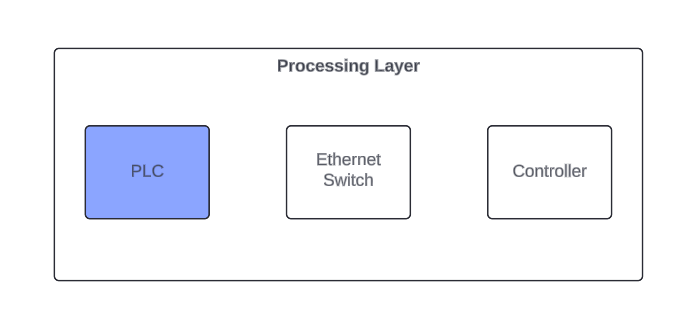
\includegraphics[width=0.60\textwidth]{images/Processing_PLC.png}
 \caption{PLC subsystem.}
\end{figure}

\subsubsection{Assumptions}
PLC is like a central processing unit of this product. The input comes from the input layer and is written onto to the PLC since the primary purpose of using a PLC is to automate the process. 

\subsubsection{Responsibilities}
The responsibility of the PLC being used in this project is to save the logical program and movement program, and to continuously process the state of the work cell. The PLC is written with a logic-based program that receives input signals from the input layer and manipulates them according to the program specification. PLC is also responsible to send output signals to other components within the system such as the air compressor and light tower to conclude the process. The output signals are computed via the logic written in the PLC. It also receives input signals from inductive switches for calibration purposes. 


\begin {table}[H]
\caption {Subsystem interfaces} 
\begin{center}
    \begin{tabular}{ | p{1cm} | p{4cm} | p{4cm} | p{4cm} |}
    \hline
    ID & Description & Inputs & Outputs \\ \hline
    \#01 & Programmable Logic Controller & \pbox{4cm}{Logic Program} & \pbox{4cm}{Send to different devices}  \\ \hline
    \#02 & Programmable Logic Controller & \pbox{4cm}{Movement Program} & \pbox{4cm}{Send to Controller}
    \\\hline
    \#03 & Programmable Logic Controller & \pbox{4cm}{Inductive switches} & \pbox{4cm}{Light Tower}\\
    \hline
    \end{tabular}
\end{center}
\end{table}

